% !TeX spellcheck = en_US

We retrieve a set of different spacial data-sets from  public sources as a basis to create the cost raster.
Field of study are the counties of Cuxhaven and Osterholz in the state of Lower Saxony, Germany.
Areas protected by different European and National conservation laws are provided by the German Environment Agency
as \acrfull{wfs}~\cite{noauthor_schutzgebiete_2015}.

The nationwide land coverage (ATKIS) with a scale of 1:250000 are provided by the Federal Agency for Cartography
and Geodesy~\cite{noauthor_digitales_2021}.
The nationwide power grid (tags: 'power': line) has been retrieved via OpenStreetMap~\cite{boeing_osmnx_2017}.
Local data as houses at Level of Detail 1 are offered by the State Office for Geoinformation and Land Surveying of
Lower Saxony\cite{noauthor_opengeodatani_2022}.
In addition, local planning geodata for the land usage are taken
from 'Metropolplaner' (Planing data Lower Saxony \& Bremen)\cite{noauthor_metropolplaner_2022}

PyWPS\cite{noauthor_welcome_2016} is used to offer the least cost path algorithm as a \acrfull{wps}.
The initial implementation of the least cost path algorithm is based on the implementation for the QGIS-Plugin
'Least Cost Path'\cite{noauthor_leastcostpathdijkstra_algorithmpy_2022} in version 1.0.

The different layers from the different entities are optionally filtered, buffered and then rasterized.
Filtering the layers of the files for special attributes enables to further differentiate.
For examples makes it possible to differentiate between heath and uncultivated land.
Adding a buffer can be used either used to convert a line objects as power grids and streets into a polygon with the
correct physical width, or to add minimum distance from an existing of planed area to the new power grid.
Each of theses rasterized layers are given a weight, or cost that expresses the cost of using land covered by this layer.
The costs of all layers of is aggregated with the maximum function.
Thus, an area covered by multiple layers is uniformly used with the highest costs.
For every area in the study area, that is not covered by any layer, is given the default cost.
The costs have been grouped into different levels~(see table~\ref{tab:1}) starting from preferential areas with
very low costs, via no restrictions, which is the default, used when no other layers are covering the local area,
to restricted, strongly restricted and prohibited areas with high costs.
These higher costs resemble the degree how much a local area should be avoided, while routing the path.
The ratio of the higher costs to the lower costs directly translates into the additional diversion in pixels
the algorithm is willing to go, for avoiding an area of high costs.
Thus, as prohibited areas describe a legal obligation, not to use these areas or only to the utmost minimum,
the weight that resembles the costs for these types of areas, has to be especially high. \\
The rasterization transforms a vector into a raster.
The rasterization can be executed in to different ways.
In both ways, the rasterization can be imaged, as the old vector is layered over the new raster grid with the new
given resolution and the new affine transformation and the coordinate reference system of the vector.
Both rasterization techniques differ in how the pixels are selected, that describe, that a geo-object overlays the pixel.
The pixels can either be described as overlaid with a geo-object, when either the center of that pixel is overlaid
by the geo-object, or any part of the pixel is overlaid.
Hence, the version with any part overlaid is called all touched True.
The version where a overlaid pixel center is require is thus called all touched False.
All touched False is considered the default (see figure~\ref{fig:alltouched}).
\begin{figure}[!ht]
	\centering

	\resizebox{8cm}{!}{
		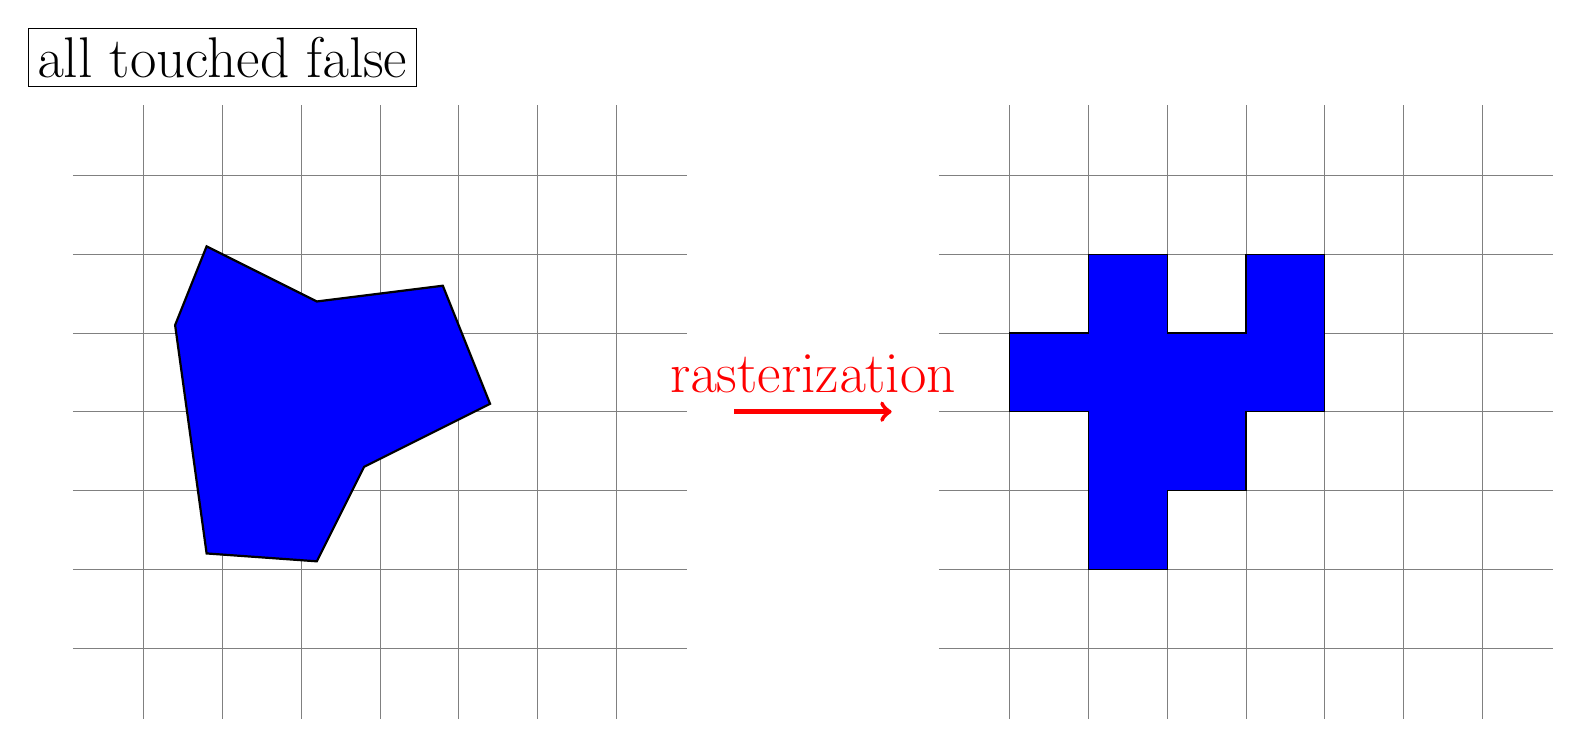
\begin{tikzpicture}
			\node[draw] at (0,6.5) {\huge all touched false};
			\draw[step=1cm,gray,very thin] (-1.9,-1.9) grid (5.9,5.9);
			\draw[fill=blue, thick] (-0.2, 0.2)--(-0.6, 3.1)--(-0.2,4.1)--(1.2,3.4)--(2.8,3.6)--(3.2, 2.6)--(3.4, 2.1)--(1.8,1.3)--(1.2, 0.1)--cycle;

			\draw[ultra thick,->, red] (6.5, 2) --node[above=1mm] {\huge rasterization} (8.5, 2);

			\draw[step=1cm,gray,very thin] (9.1,-1.9) grid (16.9,5.9);
			\draw[fill=blue] (11,0)--(11,2)--(10,2)--(10,3)--(11,3)--(11,4)--(12,4)--(12,3)--(13,3)--(13,4)--(14,4)--(14,2)--(13,2)--(13,1)--(12,1)--(12,0)--cycle;
		\end{tikzpicture}%
	}%
	\vspace*{5mm}
	\resizebox{8cm}{!}{
		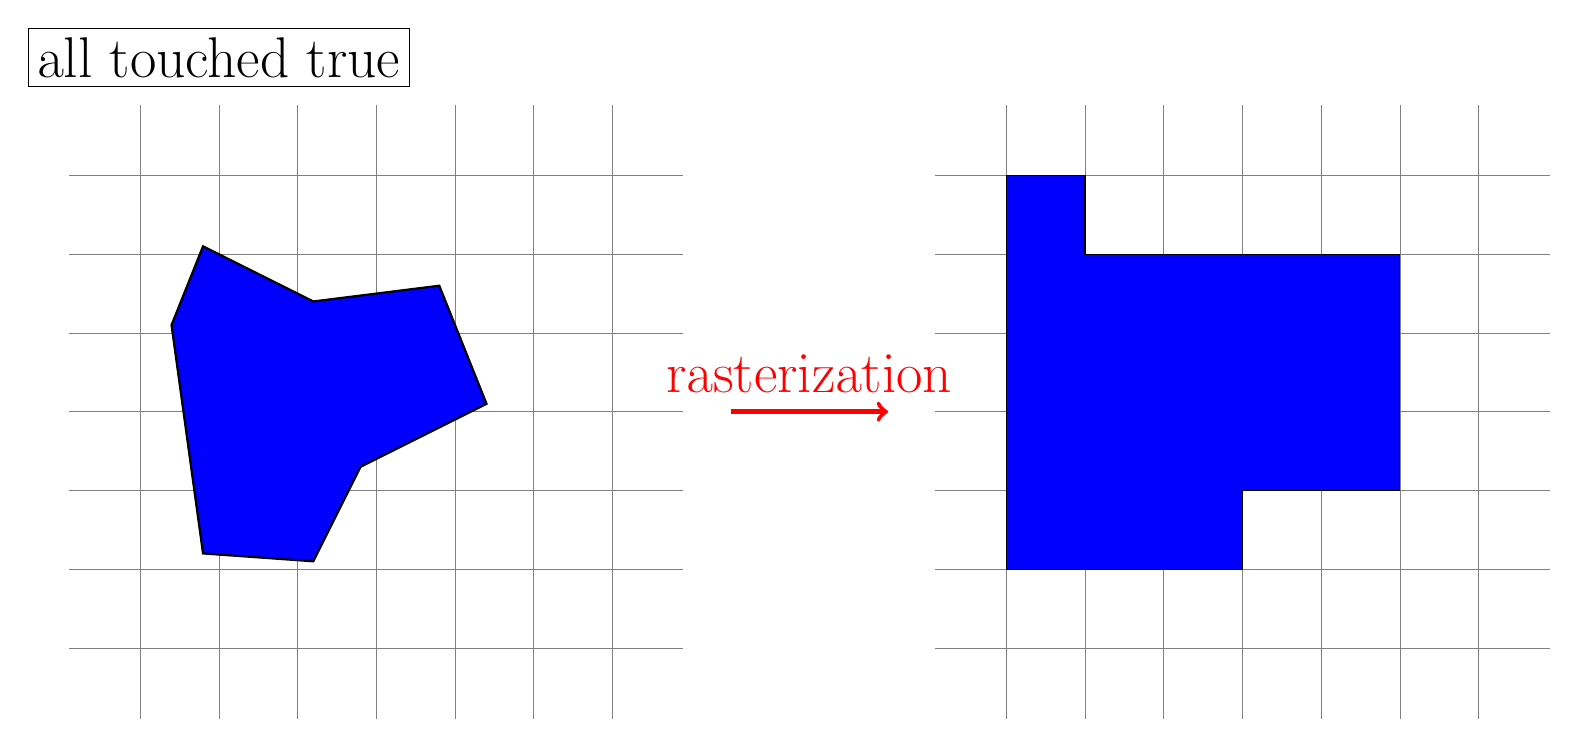
\begin{tikzpicture}
			\node[draw] at (0,6.5) {\huge all touched true};
			\draw[step=1cm,gray,very thin] (-1.9,-1.9) grid (5.9,5.9);
			\draw[fill=blue, thick] (-0.2, 0.2)--(-0.6, 3.1)--(-0.2,4.1)--(1.2,3.4)--(2.8,3.6)--(3.2, 2.6)--(3.4, 2.1)--(1.8,1.3)--(1.2, 0.1)--cycle;

			\draw[ultra thick,->, red] (6.5, 2) --node[above=1mm] {\huge rasterization} (8.5, 2);

			\draw[step=1cm,gray,very thin] (9.1,-1.9) grid (16.9,5.9);
			\draw[fill=blue] (10,0)--(10,5)--(11,5)--(11,4)--(15,4)--(15,1)--(13,1)--(13,0)--cycle;
		\end{tikzpicture}%
	}%
	\caption{Graphical example for rastering a vector (left blue), to a raster (right blue) with weither all-touched False (above), or all touched True (below).}
	\label{fig:alltouched}

\end{figure}

\begin{table}[h!]
	\caption{Used levels of costs, the applied numerical equivalent and example layer this cost have been used for.}
	\label{tab:1}
	\centering
	\begin{tabular}{ l  r  l }
		Cost Level 			& Cost 					& Example\\
		\hline
		Prohibited 			& 500					& \makecell[lt]{Conversation areas as\\ National Parks, Buildings} \\
		strongly Restricted & 10 					& \makecell[lt]{Conversation areas as Bird Reserve} \\
		Restricted 			& 5						& \makecell[lt]{Protected Landscape Area,\\ Industrial Areas, motorway, railway} \\
		No Restriction 		& 0.5					& Default\\
		Preferential 		& 0.1					& \makecell[lt]{Power Grid,\\ Motorway and Railway Buffers}\\
	\end{tabular}
\end{table}
The completed list of layers and the processing applied to them, can be found in Supplement S1. \todo{create the Supplement from the processing rules}

The whole stack of the cost raster, via the aggregated costs to the resulting least cost path can is shown with an example for a starting cost raster of 50~m resolution and a rasterization with all touched False (see \ref{fig:costs2path}).
Because of the early stopping strategy used in the aggregation sub-paths with high costs have not been fully computed.Instead the execution stops early after reaching the end point. Because the end point ends at a power transformer, which is a building type, the paths ends at in a Prohibited Area. Therefore areas even farther away from the starting point have been explored first.

\begin{figure}
	\centering
	
	\subfloat[\centering Cost Raster.]{{\includegraphics[width=.25\linewidth]{./images/CostRasterExample.png} }}%
	\qquad
	\subfloat[\centering Aggregated Cost Raster.]{{\includegraphics[width=.25\linewidth]{./images/AggregatedCosts.png} }}%
	\qquad
	\subfloat[\centering Least Cost Path.]{{\includegraphics[width=.25\linewidth]{./images/LeastCostPathExample.png} }}%

	\caption{Figures of Cost raster and the resulting aggregated Costs and the least cost path for a resolution of 50~m.}
	\label{fig:costs2path}
\end{figure}